\subsection*{Monte Carlo Sampling}

% Week 8

\begin{defe}[Empirical distribution] \label{defe: em_dist}
    Let $x_1 , \ldots , x_n$ be an iid real-valued sample from a cdf $F$. The function
    \begin{equation*}
        F_{n} (x) = \frac{1}{N} \sum_{i=1}^{N} \Id_{\left\{ x_i \leq x \right\}} (x) , \quad x \in \RR
    \end{equation*}
    is called the {\bf empirical cdf} of the data \cite{KroeseDirkP2013SMaC}*{page 196}.
\end{defe}

\begin{figure}[ht]
    \centering
    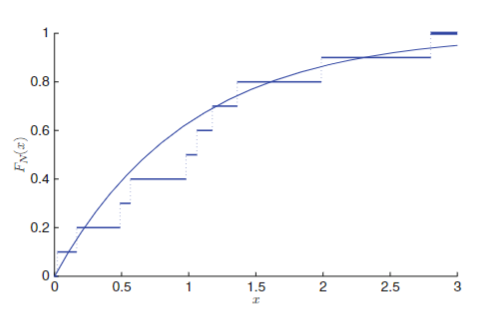
\includegraphics[scale=1.0]{img/bay_inf/emp_cdf_exp_1.png}
    \caption{The empirical cdf \ref{defe: em_dist} for a sample size $10$ from a $\Exp (0.2)$ distribution as well as the true cdf. Image from \cite{KroeseDirkP2013SMaC}*{page 197}.}
    \label{fig: emp_cdf_exp_1}
\end{figure}

Note that for the ordered sample $x_{(1)} < x_{(2)} < \cdots < x_{(N)}$,

\begin{equation*}
    F_{N} \left( x_{(i)} \right) = \frac{i}{N}.
\end{equation*}

assuming for the sake of simplicity that all $\left\{ x_i \right\}$ take on different values. If instead of deterministic $\left\{ x_i \right\}$ we take random $X_i$, then $F_N (x)$ becomes random as well. To distinguish between the deterministic and the random case, let us denote the random empirical cdf by $\hat{F}_{N} (x)$. We now have
\begin{equation*}
    \PP \left[ \hat{F}_{N} (x) = \frac{i}{N} \right] = \PP \left[ X_{(i)} \leq x , X_{(i+1)}  x \right] = \binom{N}{i} \left( F(x) \right)^{i} \left( 1 - F(x) \right)^{N-i}
\end{equation*}
\cite{KroeseDirkP2013SMaC}*{page 198}. The above equation can be summarized as $N \hat{F}_{N} (x) \sim \Bin (N, F(x))$. Consequently,
\begin{align*}
    \EE \left[ \hat{F}_{N} (x) \right]  & = F(x)                          \\
    \Var \left[ \hat{F}_{N} (x) \right] & = F(x) \left( 1 - F(x) \right).
\end{align*}
Moreover, by the law of large numbers and the central limit theorem, we have
\begin{equation*}
    \PP \left[ \lim_{N \to \infty} \hat{F}_{N} (x) = F (x) \right] = 1,
\end{equation*}
and
\begin{equation*}
    \lim_{N \to \infty} \PP \left[ \frac{\hat{F}_{N} (x) - F(x)}{\sqrt{F(x)(1-F(x)/N)}} \right] = \Phi (z).
\end{equation*}

\begin{defe}[Confidence Intervals] \label{defe: confd_int}
    Let $X_1 , \ldots , X_n$ be random variables with a joint distribution depdending on a parameter $\theta \in \Theta$. Let $T_1 < T_2$ be functions of the data but not of $\theta$. The random interval $(T_1 , T_2)$ is called a {\bf stochastic confidence interval} for $\theta$ with confidence $1 - \alpha$ if
    \begin{equation*}
        \PP_{\theta} \left[ T_1 < \theta < T_2 \right] \geq 1 - \alpha \quad \text{for all} \quad \theta \in \Theta.
    \end{equation*}
    If $t_1$ and $t_2$ are the observed values of $T_1$ and $T_2$, then the interval $(t_1 , t_2)$ is called the {\bf numerical confidence interval} for $\theta$ with confidence $1 - \alpha$ \cite{KroeseDirkP2013SMaC}*{page 128}.
\end{defe}

An approximate $1 - \alpha$ confidence interval for $F(x)$ is
\begin{equation*}
    F_N (x) \pm z_{1 - \alpha / 2} \sqrt{\frac{F_N (x) (1 - F_N (x))}{N}}
\end{equation*}
where $z_{1 - \alpha / 2}$ is the $1 - \alpha / 2$ quantile of the standard normal distribution. Moreover for the ordered sample $x_{(1)} < x_{(2)} < \cdots < x_{(N)}$, an approximate $1 - \alpha$ confidence interval for $F(x_{(i)})$ is
\begin{equation*}
    \frac{i}{N} \pm z_{1 - \alpha / 2} \sqrt{\frac{i(1 - i/n)}{N^2}}
\end{equation*}
\cite{KroeseDirkP2013SMaC}*{page 198}.

\subsubsection*{Simultaneous Confidence Bands}

% Week Lec 2, Ch 7.1

\begin{defe}[Kolmogorov–Smirnov statistic] \label{defe: TBD}
    For a continuous $F$, the statistic of
    \begin{equation*}
        D_n = \sup_{x \in \RR} \left| \hat{F}_N (x) - F(x) \right|
    \end{equation*}
    is called the {\bf Kolmogorov–Smirnov statistic} \cite{KroeseDirkP2013SMaC}*{page 200}.
\end{defe}

Note that this statistic does not depend on $F$ and can be used to test whether iid samples $X_1 , \ldots , X_n$ come from a specified distribution as well as constructing a simultaneous confidence band for $F$. The empirical cdf can be used to estimate any cdf, both discrete and continuous, but it is always 'jumpy' which may be undesirable, for example when the underlying distribution is continuous. When we have continuous data, we may want a continuous density estimate instead. This leads to our next topic of density estimation.

\subsubsection*{Kernel Density Estimation}

\begin{defe}[Kernel Density Estimator] \label{defe: KDE}
    Let $X_1 , \ldots X_n \iid f$ from a continuous distribution with cdf $F$. A {\bf Kernel density estimator} (KDE), also known as a sliding window estimator, with bandwidth $h$ is given by
    \begin{equation*}
        \hat{f} (x;h) = \frac{1}{N} \sum_{i=1}^{N} K \left( \frac{x_i - x}{h} \right).
    \end{equation*}
    The function $K (\cdot)$ is the kernel function ("window shape") and $h$ is the window ("window size").
\end{defe}

There are many choice of $K$, but we shall just focus on the Gaussian kernel.

\begin{defe}[Gaussian Kernel] \label{defe: gauss_kern}
    The {\bf Gaussian Kernel} uses a kernel of
    \begin{equation*}
        K(x) = \frac{1}{\sqrt{2 \pi}} \exp \left( - \frac{1}{2} x^2 \right)
    \end{equation*}
    so that
    \begin{equation*}
        \hat{f} (x;h) = \frac{1}{N} \sum_{i=1}^{N} \frac{1}{\sqrt{2 \pi}} \exp \left( - \frac{1}{2} \left( \frac{x_i - x}{h} \right)^2 \right)
    \end{equation*}
    \cite{KroeseDirkP2013SMaC}*{page 201}.
\end{defe}
% Week 9 content
Essentially, the Gaussian kernel is just an equally weighted $\frac{1}{N}$ normal mixture model. It has $N$ Gaussian "humps", centered at each observation and has standard deviation $h$. As it turns out, the choice of the kernel is not that crucial, but the choice of the bandwidth is very important. An often used {\it rule of thumb} is to take
\begin{equation*}
    h_{\text{Rot}} = \left( \frac{4S^5}{3N} \right)^{4/5}
\end{equation*}
called the Silverman's rule of thumb where $S^2$ is the variance. This is based on a theoretical analysis of the discrepancy between $f_n (x;h)$ and the true pdf, as $n \to \infty$. This rule f thumb is best suited when the underlying data is roughly normal-looking (i.e unimodel and symmeteric). A more recent bandwidth selection methods \cite{10.1214/10-AOS799}, called the theta KDE, adaptively changes the bandwidth.

\subsubsection*{Bootstrap Method}

A key concept in statistics is the idea of a sampling distribution (i.e. the distribution of the sample quantity, if we could repeat the random experiment over and over again). Unfortunately, we typically only get one realization of the random process, from which we compute sample quantity we want (for example the sample mean or medium). So, how can we get a feel about the sampling distribution if we have only one realization?

\begin{exam}[Bootstrap Median] \label{exam: bootstrap_median}
    Suppose we have the following sample
    \begin{equation*}
        6.45 , 3.52 , 3.92 , 0.64 , 3.73 , 2.00, 2.73 , 4.20, 20.58, 6.80, 3.22, 7.11, 1.08 , 5.94.
    \end{equation*}
    From this data, how do we construct a confidence interval for the true population medium $M$ of the distribution $F$ that generated the data? Ideally we sample from $F$ over and over again and each time we compute the sample medium and then we look at the distribution of the computed sample medians. Since we don't have access to the distribution $F$, we can instead employ the bootstrap method.
    \begin{itemize}
        \item To start we take iid sample of size $n$, $x^{\ast}$, from the empirical cdf $F_n$ with replacement.
        \item For each sample, we compute the sample medium $m^{\ast}$ of the resampled data.
        \item Then we look at the $2.5$ percentile and the $97.5$ percentile of the resampled values of the mediums.
        \item This percentiles together provide an approximate $95$ percent confidence interval for the population median $M$.
    \end{itemize}
\end{exam}

We can use the bootstrap method to estimate any property of the sample distribution, for example, the variance of the sample mean, medium or IQR. In general we may be interested in some property $h$ (eg. bias, variance, MSE) of some statistic $H(\bm{x})$ (eg. median, $\frac{1}{\overline{X}}$) we can apply the bootstrap resampling approach to estimate these properties.

    {\centering
        \begin{minipage}{.85\linewidth}
            \begin{algorithm}[H]
                \caption{Bootstrap Method}
                \label{alg: bootstrap}
                \SetAlgoLined
                \DontPrintSemicolon
                \SetKwInOut{Input}{input}\SetKwInOut{Output}{output}

                \Input{Observations $\bm{X}, \bm{y}$ and a test input $\bm{x}_{\star}$.}
                \Output{A prediction $\overline{f_{\star}} $ with its corresponding variance $ \VV \left[ f_{\star} \right]$.}
                \BlankLine
                \For{$i\gets 1 , \ldots , K$}{
                Resample data $x_1^{\ast} , x_1^{\ast}, \ldots , x_n^{\ast}$ from the original data.\;
                For each sample, calculate $h(H_k^{\ast}) = h(H(x_k^{\ast}))$\;
                }
                Estimate $\EE \left[ h(H(x)) \right]$ using $\frac{1}{K} \sum_{i=1}^{K} h(H_k^{\ast})$
                \BlankLine
            \end{algorithm}
        \end{minipage}
        \par
    }

For example to compute the variance of the sample medium we can compute
\begin{equation*}
    \VV (\text{medium}) = \EE \left[ (m - \EE(m)) \right]^2 \simeq \sum_{i=1}^{K} (m_i^{\ast} - \overline{m}^{\ast})^2
\end{equation*}
where $m_i^{\ast}$ is the sample median of the ith resampled dataset and $\overline{m}^{\ast}$ is the mean of the resampled median values.